\begin{quote}
\begin{center}
	\textfill{שוויון וצדק \textbf{לכולם}, מהירדן ועד הים}\\
	%\textfill{שִׁוְיוֹן וְצֶדֶק לְכֻלָּם, מֵהַיַּרְדֵּן וְעַד הַיָּם}\\
	%\textfill{\Ar{المساواة و العدالة \textbf{للجميع} من نهر الأردن إلى البحر}}
	\textfill{\Ar{مساواة و عدالة \textbf{للجميع} من نهر الأردن إلى البحر}}
\end{center}

לא שוויון, לא חירות, לא צדק ולא זכויות־אדם בסיסיות יש בין הירדן והים. הגורם העיקרי שֶׁמְּתַחְזֵק את המצב הלא־צודק הזה הוא \hl{מדינת־ישראל}, המוּנעת מאידיאולוגיה גזענית־ציונית ומתאוות־בצע קפיטליסטית.

\hl{זה לא צריך להיות ככה; יום יבוא וזה לא יהיה ככה \smaller{(רק אם נפעל לשינוי)}}. כמו האפרטהייד בדרום־אפריקה, תיפול ההפרדה הגזעית כאן; כמו חומת ברלין, תיפול גם חומת ההפרדה כאן.

%***זכות ההפגנה (לפלסטינים אין) והאלימות המשטרית
%***פליטים
%***חינוך: הפרדה (דת + שפה) + לאומנות
%***גבעת עמל. הון־שלטון. ויתור על חובות ומסים
%***טיהור אתני
%***חוק השבות וחוגי גזע בכלל
%איפה אתם בסגר?
%פראוור
%גיוס חרדים

{\small כדי לקרוא את ה\hl{מקורות} אליהם אני מפנה, צריך להוסיף לפני התוכן של הסוגריים המרובעים (ללא הסוגריים) {\url{http://bit.ly/}}. מקורות מידע כלליים:
האגודה לזכויות־האזרח (\url{acri.org.il}), הטלוויזיה החברתית (\url{tv.social.org.il}), בְּצֶלֶם (\url{btselem.org}).}
\end{quote}

\hrule

בקרוב~— ב־6 במאי השנה~— יציינו רבים את „יום־העצמ{\small א}ות”, ורבים אחרים (בעיקר ב־15 במאי, ר׳ \reference{cYvNlK}{http://en.wikipedia.org/wiki/Nakba_Day}) את „יום־הנכבה” (\Ar{يوم النكبة}). \hl{זה זמן מצויין לעצור ולחשוב} על החברה שבה אנחנו חיים ועל מה שעושה מדינת־ישראל בשמנו ובעזרת כספנו.

{\setlength\parindent{-0.5em}\Large אנחנו חיים במדינה~—}

%\begin{itemize}
	\vspace{-0.35em}
% \setlength{\itemsep}{1pt}
	\bull{\hl{שוללת} זכויות־אדם ו\hl{מפלה} בכל תחומי־החיים מליוני אנשים לפי מוצאם}
	\bull{יש בה \hl{דין שונה}~— דה־יורו ודה־פקטו~— לאנשים ממוצא שונה, הן בגבולות 67׳ והן בגבולות 48׳. בגבולות 67׳ אנשים ממוצא פלסטיני נתונים תחת חוק צבאי, ואנשים ממוצא יהודי תחת חוק אחר, אזרחי \smaller{(כך, כדוגמה אחת מרבות מספור, לאלה אסור להפגין ולאלה מותר (צו 101: \reference{1fh8nlR}{http://www.btselem.org/hebrew/demonstrations/military_law}))}}
	\bull{\hl{מענה ומתעללת} בנחקרים ועצירים \reference{9YoUpE}{http://www.stoptorture.org.il}}
	\bull{בה המשטרה יכולה, אפילו בלי צו בית־משפט, לקבל נתונים על תקשורת אלקטרונית, ומבלי שתהיה אפשרות למי שהמשטרה \hl{מרגלת} אחריו לדעת את זה \reference{br90tu}{wiki} \smaller{(למשל, המיקום שבו נמצא טלפון נייד בעת שיחה וזהות המשתתפים בשיחה, ונתונים על גלישה באינטרנט והתכתבות בדואל (הגנה חלקית: \reference{28eq6j}{http://en.wikipedia.org/wiki/Tor_(anonymity_network)}))}, }
	\bull{מבצעת \hl{פשעי־מלחמה} על בסיס יומיומי \smaller{(דוגמאות לפשעי־מלחמה: הוצאות־להורג ללא משפט („חיסולים”), עינויים והתעללות, ענישה קולקטיבית („סגר”, „חישוף”), הריסת־בתים כענישה, הפקעת אדמות ובתים, מניעת אספקת מזון וטיפול רפואי, שימוש בכלי־נשק שלא מאפשרים הבחנה בין חיילים ואזרחים ועוד…)} \reference{1rqI2n3}{http://www.yeshgvul.org.il/notebook/} \reference{deubWz}{http://www.shovrimshtika.org/}}
	\bull{מרשתת את הרחובות בה ב\hl{מצלמות מעקב} ויתכן שיוקם בה \hl{מאגר זיהוי ביומטרי בכפיה} בעתיד הקרוב \reference{1kancoW}{http://no2bio.org/}}
	\bull{\hl{מדכאת} בכח הזרוע \hl{מחאה} עממית בלתי־אלימה נגד עוולות שהיא מבצעת \smaller{(אלות, טייזרים, מעצרים, רימוני ופצצות גז מדמיע, רימוני הלם, כדורי מתכת מצופים שכבת גומי ושאינם מצופים, התזת כימיקלים מצחינים („הבואש”), החרשת־אוזניים („הצעקה”), פשיטות ליליות \reference{1mdeKpw}{http://972mag.com/watch-army-raids-three-west-bank-villages-arrests-activists/87420/}, ועוד)}, אפילו תוך הפרת חוקי הצבא הישראלי עצמו \reference{1kbvfSr}{http://www.btselem.org/hebrew/firearms/20120422_direct_firing_of_tear_gas_continues}. \smaller{פרקטיקה רגילה היא לירות ולהשפריץ ללא הבחנה על רחובות ובתים בכפרים שמקיימים הפגנות, כדי ליצור סכסוכים פנימיים}}
	\bull{\hl{רודפת פעילים} לזכויות־אדם \reference{bzt7cD}{http://www.btselem.org/Hebrew/Press_Releases/20100202.asp} \reference{1lN29Z7}{http://www.acri.org.il/he/2394} \reference{1laPVv4}{http://www.ynet.co.il/articles/0,7340,L-3576974,00.htmlhh} \reference{1k7IzFP}{http://www.haaretz.co.il/opinions/editorial-articles/1.2305452}}
	\bull{\hl{מפרה} דרך קבע \hl{אמנות} והכרזות שהיא חתומה עליהן \smaller{(לדוגמה: ההכרזה לכל־באי עולם בדבר זכויות־האדם \reference{c60wSr}{he.wiki} ואמנות־ז׳נבה \reference{cFPvPQ}{he.wiki})}, כמו גם את חוקיה־שלה (כשנוח ומתאים לה…) וחוקים בינלאומיים}
	\bullclean{יוצאת ל„\hl{מלחמות יש ברירה}” שהן רוויות־דם וממיטות הרס עצום על תשתית אזרחית. \smaller{מהשנים האחרונות:
			\vspace{-1.00em}
			\begin{itemize}
				\item בהתקפות על \hl{הלבנונים ב־{2006}} \reference{9jTzZY}{wiki}~— \numdata{300–450} אזרחים נרצחו בלבנון (45\% מסה״כ שם), כ־\numdata{2,500} אזרחים נפצעו וכ־\numdata{1,000,000} אזרחים נעשו פליטים (רבע מאוכלוסיית לבנון); במדינת־ישראל: \numdata{44} אזרחים נרצחו וכ־\numdata{2,000} אזרחים נפצעו.
				\item בהתקפות על \hl{העזתים ב־{2008}} \reference{bH2OWl}{wiki} \reference{d9xxa8}{http://www.btselem.org/Hebrew/Gaza_Strip/20091227_A_year_to_Castlead_Operation.asp} \reference{1fkSNFv}{http://idanlandau.com/2009/12/25}~— \numdata{762} אזרחים נרצחו בעזה (55\% מסה״כ שם; \numdata{318} קטינים), למעלה מ־\numdata{5,300} אזרחים נפצעו (למעלה מ־\numdata{350} קשה) וכ־\numdata{20,000} אזרחים נותרו ללא קורת־גג; במדינת־ישראל: \numdata{3} אזרחים נרצחו ו־\numdata{183} אזרחים נפצעו (\numdata{28} קשה).
				\item בהתקפות על \hl{העזתים ב־{2012}} \reference{PGRftg}{http://idanlandau.com/2013/05/10/pillar-of-smokescreen-the-real-numbers/} \reference{1lVOMpz}{http://www.btselem.org/download/201305_pillar_of_defense_operation_heb.pdf}~— \numdata{87} אזרחים נרצחו בעזה (52\% מסה״כ שם; \numdata{34} ילדים) ו־\numdata{970} אזרחים נפצעו; במדינת־ישראל: \numdata{4} אזרחים נרצחו ו־\numdata{240} אזרחים נפצעו
			\end{itemize}
			\vspace{-0.50em}
	}}
	\bull{סוגרת את שעריה ל\hl{פליטים ומבקשי־מקלט} שנסים על נפשם בעזרת גדר בדרום וציידי־אדם, שולחת רבים מהם חזרה, גם כאשר צפויה להם סכנת־חיים \reference{b6mYQb}{http://www.amnesty.org.il/?CategoryID=170}, וכולאת רבים מהם ב„חולות” וב„סהרונים” בתת־תנאים}
	\bull{מטילה \hl{מצור} של חנק על יותר מ־\numdata{1,800,000} אנשים ב\hl{עזה} \smaller{(המכונה גם „הכלא הגדול ביותר בעולם”)}, מהם כ־\numdata{1,000,000} פליטים, שכמחציתם מתגוררים במחנות־פליטים \reference{c6tDyi}{he.wiki}: מניעה של יבוא מוצרים שונים \smaller{(מכלי־נגינה \reference{1rzKzvm}{http://gisha.org/he-blog/2010/01/05} ועד חומרי־בניין (בין השאר לשיקום ההרס מ־2008 ו־2012…) \reference{1lVQA6z}{http://gisha.org/he-blog/2014/01/29})}, מניעה של אספקת תשתית למחיה \smaller{(מים, חשמל, דלק וכו׳; בעניין: סרט \reference{buZpRF}{http://he.reutsadaka.org/?p=1138})} ומניעה של כניסה ויציאה מ־/אל עזה.\\
		\smaller{הידעת? 80\% מהאנשים שחיים בעזה תלויים בסיוע בינלאומי למחייה \reference{1nxke1n}{http://www.ipsnews.net/2010/07/mideast-israel-chokes-gaza-despite-announced-easing/}}}
	\bull{בחסותה ובעזרתה \hl{קבוצה דתית אחת כופה} את דרכיה על שאר האוכלוסיה, במגוון תחומים בחיים \reference{1jW7X04}{https://he.wikipedia.org/wiki/…}\\
	\smaller{חילונים ממוצא יהודי~— הידעתם? רוצים לאמץ ילד שלא מוגדר על־ידי המדינה כיהודי? תצטרכו להמיר את אי־דתכם ליהדות אורתודוקסית \reference{1kib8lz}{http://www.haaretz.co.il/1.1732976}}}
	\bull{כשליש מהתושבים בעיר־הבירה שלה \hl{נטולי־אזרחות}: מעמד „תושבי־הקבע” שלהם עומד תמיד בסכנה \smaller{(לימודים בחו"ל או מעבר־דירה, אי „הוכחת מגורים” באמצעות תשלום־מיסים, ועוד)} \reference{9zZ5M5}{http://www.btselem.org/Hebrew/Jerusalem/Revocation_of_Residency.asp}; הם אינם מקבלים באופן שיוויוני שירותי עירייה \smaller{(מלבד, כמובן, שירותי גביית־מיסים…)}, רפואה וחינוך \smaller{(חסרות כ־2,200 כיתות \reference{1iqnGJd}{http://www.ir-amim.org.il/he/report/…})}; לא מאושרת להם בניה \reference{9oYuDb}{http://www.btselem.org/Hebrew/Jerusalem/Discriminating_Policy.asp} וקרקעותיהם נגזלות, ולכן על בתיהם שנבנו בלית־ברירה בלי אישורים מרחפת סכנת־הריסה. ההתעמרות הזאת היא הצד הממסדי של הטיהור האתני הזוחל בירושלים.\\
	\smaller{הידעת? בשנת 2009 בשכונת שיח׳ ג׳ראח פונו מביתן ארבע משפחות ממוצא פלסטיני, פליטים מ־48׳ וצאצאיהם שגרו שם יותר מ־50 שנים, בתוקף מסמכים טורקיים של אנשים ממוצא יהודי על שטח הבתים, מסמכים מלפני כ־130 שנים; למסמכים כאלה ממש על שטחים בגבולות 48׳, כאשר מחזיקים בהם אנשים ממוצא פלסטיני (כמו מסמכים שבידי המשפחות הנ״ל), אין כמובן תוקף מבחינת מדינת־ישראל \reference{QS0c3H}{http://idanlandau.com/2009/10/31} \reference{1mNAF7g}{http://www.justjlm.org/about-2/…}). חפשו גם „חוק הסדרי משפט ומנהל” ו„חוק נכסי נפקדים”}}
	\bull{מטילה \hl{צנזורה} וצווי איסור־פרסום \reference{9pkj48}{http://israblog.nana10.co.il/blogread.asp?blog=97762&blogcode=11700988} \smaller{(ואולי איסור־פרסום על זה שיש איסור־פרסום על משהו… אין לדעת…)}, שאין בה חופש עיתונאי מלא \smaller{(עיתונאים ישראליים בעזה? חו״ש! נטיל צו צבאי נגד זה \reference{1lX2sAT}{http://www.haaretz.com/print-edition/opinion/the-idf-s-shooting-range-1.114011} \reference{cKJan4}{http://www.the7eye.org.il/interviews/Pages/231108_amira_hass_in_gaza.aspx})} ושעיתונאים בה נרדפים \reference{9ysgTl}{http://www.haaretz.co.il/hasite/spages/1161943.html} \smaller{(במיוחד אם, לא עלינו, מוצאם פלסטיני \reference{1rujWI9}{http://www.acri.org.il/he/31181})}}
	\bull{הוקמו בה, במקרים רבים בסיועה, 600 „\hl{ישובים יהודיים}”, מול \hl{עיירות ספורות} בלבד עבור אנשים ממוצא פלסטיני \smaller{(כולן עם תשתית ותקצוב ירודים)} \reference{1k96IvJ}{http://www.acri.org.il/he/1783}, ובעוד שאין תוכניות־פיתוח עדכניות ומתאימות עבור ישובים שבהם האוכלוסיה ממוצא פלסטיני \reference{9oYuDb}{http://www.btselem.org/Hebrew/Jerusalem/Discriminating_Policy.asp} \reference{cfrGGt}{http://www.btselem.org/Hebrew/Planning_and_Building/Index.asp} \reference{908xlo}{http://news.walla.co.il/?w=//1392369}, הרס־הבתים נמשך במלוא־הקצב, וקרקעות פרטיות נגזלות \reference{asxTQu}{http://www.haaretz.com/hasite/spages/1059834.html}}
	\bull{(על־פי פרסומים זרים…) מחזיקה ב\hl{כלי־נשק להשמדה המונית} \reference{10eNew}{http://en.wikipedia.org/wiki/Israel_and_weapons_of_mass_destruction} \smaller{(לא, בדימונה זה לא מפעל־טקסטיל)}}
	\bull{מונעת אספקת \hl{מים} סדירה (או בכלל) לאנשים ממוצא פלסטיני \reference{9yMxuS}{http://www.haaretz.com/hasite/spages/1105703.html} \reference{dz5krP}{http://www.btselem.org/Hebrew/Water/Index.asp} \smaller{(תמהתם פעם למה משמשים הדודים השחורים על גגות־הבתים?)}. פעם יש, פעם אין ופעם המים לא נקיים}
	\bull{\hl{החריבה} יותר מ־\numdata{18,000} \hl{בתים} של אנשים ממוצא פלסטיני מאז 1967 \smaller{(זה יוצא כ־\numdata{8} בתים בשבוע בממוצע; \numdata{8} משפחות שחרב להן ביתן, בכל שבוע)}}
	\bull{מקימה מאז 2002 \hl{חומת־אפרטהייד} \smaller{(אגב, הידעת? פירוש המילה „\L{Apartheid}” בלשון אפריקנס היא… „הפרדה” (תרגום מילולי לאנגלית יהיה \L{apart-hood}))} שרק עליה אפשר למלא הרבה מאוד דפים כמו זה. הרס, הגבלת־תנועה, גזל־קרקעות ומשאבים \smaller{(הגזלת וגם בנית חומה באמצעות הגזל? ר׳ מהדורה 39 של \reference{zQxxB}{http://www.hayarkon70.org/})} ופגיעה בחקלאים, פירוד, „ניהול” אוכלוסיה אזרחית ונסיון לשבירת־רוח הם רק חלק קטן מהביטויים המתאימים כאן. \smaller{הרשויות המבצעות מצפצפות על הרשות השופטת לא רק במעצר בלתי־חוקי של מפגינים, לדוגמה, אלא גם בעניין תוואי־החומה}}
	\bull{חצי משטח „קרקעות־המדינה” בה הם \hl{שטחים צבאיים} \reference{cwikcK}{http://www.themarker.com/tmc/article.jhtml?ElementId=skira20081114_1037135} \smaller{(תסתכלו במפה שם: 9,000,000 דונם, שליש משטח מדינת־ישראל, מוגדרים כשטחי אימונים וניסויים של הצבא)}}
	\bull{יש בה \hl{חוק גיוס חובה}, שכופה על אנשים לקחת חלק בארגון צבאי, ובפרט בכזה המבצע פשעי־מלחמה \smaller{(אגב, מצד שני, כמה נתונים לגבי אי־גיוס (מי אמר „צבא־העם”?): לפי ראש אגף כוח־אדם בצבא הישראלי 44\% מהנקבות ו־25.8\% מהזכרים שב„פוטנציאל הגיוס” לא מתגייסים; 17\% מהזכרים מתגייסים אבל עוזבים לפני תום שלוש־השנים של עבודות־הכפיה (המקור, \reference{9hVgwv}{http://www.ynet.co.il/articles/0,7340,L-3679285,00.html}, פרו־מיליטריסטי, אבל הנתונים הם העיקר כאן). מחישוב שנעשה ב־2005 עולה ש־46\% מכלל בני ובנות ה־18 לא מתגייסים \reference{b1QIG4}{http://www.notimportant.co.il/wp-content/uploads/itamar/gonzo-guide-for-young-kabanists-21.pdf})}. אגב, הידעת? התאבדות של חיילים היא סיבת־המוות מספר אחת בצבא הישראלי (רפרנס: \reference{91xumY}{http://www.nrg.co.il/online/1/ART/947/550.html}). בעניין־הגיוס: מוזיקה \reference{cpPEyi}{http://www.pigle.com/21/}, עזרה \reference{aHerQz}{http://www.newprofile.org/} \reference{dAYfkv}{http://www.yeshgvul.org.il/} ומידע \reference{b1QIG4}{http://www.notimportant.co.il/wp-content/uploads/itamar/gonzo-guide-for-young-kabanists-21.pdf}}
	\bull{מנסה לשמור על „\hl{טוהר הדם} היהודי” על־ידי איסור על נישואין בין־דתיים: אפילו אנשים שהם אתאיסטים מוחלטים משוייכים (לעניין זה ולעניינים נוספים) באופן גזעני לדת מסויימת לפי מוצאם \reference{bqyyah}{he.wiki}}
	\bull{פוגעת פגיעה אנושה ב\hl{חופש־התנועה} של 3,500,000 אנשים ממוצא פלסטיני בגדה המערבית, באמצעים שונים (מחסומים, כבישים ומערכת תחבו״ץ נפרדים לפי גזע, ועוד), הן בתוך הגדה המערבית והן לחוץ \reference{dny1Sa}{http://www.btselem.org/Hebrew/Freedom_of_Movement/Index.asp}. \smaller{בשנת 2006 הוטל סגר מוחלט בסה"כ 78 ימים (יותר מחמישית מהשנה) ובשנת 2005 בסה"כ 132 ימים (יותר משליש) \reference{cZHkJL}{http://www.btselem.org/Hebrew/Freedom_of_Movement/Siege_Figures.asp}\smaller{, כאשר 305,000 האנשים ממוצא יהודי שמתגוררים שם יכולים לנוע בחופשיות, כמובן}.} הפגיעה בחופש־התנועה משמעותה גם פגיעה בכל תחומי־החיים: בריאות, פרנסה, השכלה, וכו׳ \smaller{(חשבו מה קורה לגוף אם מפסיקים את זרימת־הדם…)}}
	\bull{מכבידה את עולה, מנצלת באופן שיטתי ופוגעת ב\hl{מהגרי־עבודה} ומשפחותיהם \reference{c0LpFU}{http://www.hotline.org.il/hebrew/index.htm} \reference{9SHwsR}{he.wiki}}
	\bull{מדורגת שלישית בעולם בהיקף \hl{עסקאות נשק ליצוא}, כולל פצצות מצרר \reference{1ruQpfw}{http://www.globes.co.il/news/article.aspx?did=1000503033}, ומכרה נשק למשטרים רודניים שטבחו בעשרות־אלפים \reference{aY4cCk}{abc}}
	\bullclean{מדורגת במקום הראשון המפוקפק ב\hl{מדד המיליטריזציה העולמי} (\L{Global Militarization Index}), המודד את היחס בין ההוצאות הצבאיות של מדינות לבין התוצר המקומי הגולמי (תמ״ג) \reference{1h39XTd}{http://gmi.bicc.de/}. נחשו איזה משרד נמצא בראש התקציב של 2014, עם ₪50,852,073,000 (11\%) \reference{1khUgvt}{http://budget.msh.gov.il/}…}
	\bull{מפרידה בין אנשים וחוצצת ביניהם ב\hl{עופרת, בטון ודיו}}
	\bullclean{חוברת קטנטנה כזאת לא מספיקה כדי לתאר אלא חלק קטן מהעוולות שהיא עושה…}
%\end{itemize}

\setlength\parindent{0cm}

\vfill

\textfill{לאור כל אלה, האם נשתוק ולא נפעל לשינוי יסודי בחברה בה אנחנו חיים?}

\vfill

\begin{quote}
	אני פונה אליך בבקשה \hl{לעשות מה שביכולתך} כדי להפוך את המקום שאנחנו חיים בו לפחות גזעני, פחות מיליטריסטי, פחות אלים, פחות מפלה ופחות קונפורמיסטי: בסירוב לקחת חלק בעוול (\BH{ס֣וּר מֵ֭רָע}) ובפעולה נגדו (\BH{וַעֲשֵׂה־ט֑וֹב}). שינוי משמעותי לא בא מפתק בקלפי אחת לכמה שנים, הוא בא מפעולות של האנשים עצמם. יש מקום לתקווה.~\hfill\pbox[t]{100cm}{\fontspec{Cafe}בתודה על הקריאה,~{\fontspec{Symbola}☺}\\יודה רונן}
\end{quote}

\vfill

\larger{~\hfill{\fontspec{Symbola}☜}\hfill{להצטרפות לפעולות מאורגנות גשו אל \url{http://tiny.cc/actleft}}\hfill{\fontspec{Symbola}☞}\hfill~}

\vfill


\begin{center}
	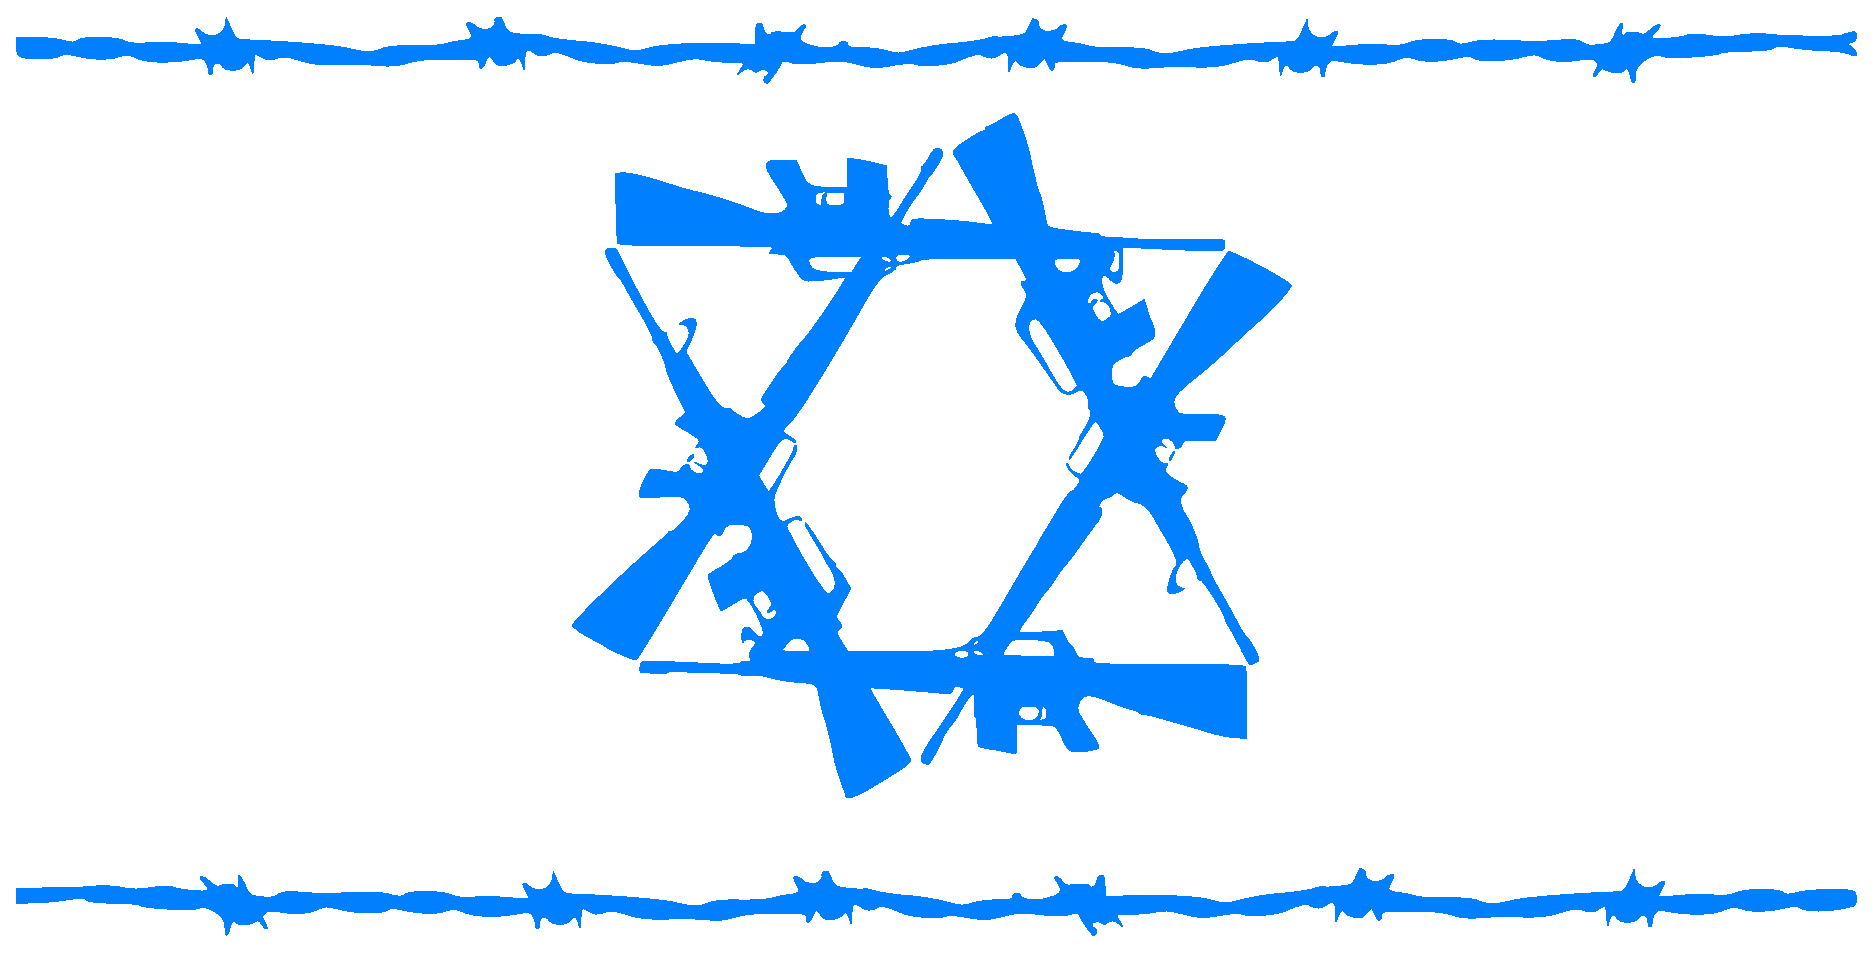
\includegraphics[width=0.6\linewidth]{flago.eps}
\end{center}

\vfill

\hrule

~\hfill לשאלות, ולדיווח על טעויות ומידע עדכני יותר: \LR{\url{nakbooklet★digitalwords.net}}\hfill~

\small הערה: יש עוולות רבות מתחומים אחרים שמקומן בחוברת מצומצם (קפיטליזם, לדוגמה) או שלא קיבלו מקום כלל (מעורבות המדינה בפגיעה בבעלי־חיים לא אנושיים, לדוגמה). אין בכך כדי להפחית, חו״ח, מחשיבותן: \BH{לַכֹּ֖ל זְמָ֑ן וְעֵ֥ת לְכָל־חֵ֖פֶץ תַּ֥חַת הַשָּׁמָֽיִם}, והחוברת הזאת מתמקדת בהיבטים של ההפרדה הגזעית.
